%\documentclass{article}

%\usepackage{graphicx}
%\usepackage{enumitem}

%\begin{document}

% Nama Kelompok : Kelompok 2
% Kelas : D4 TI 1A
% 1. Kadek Diva Krishna Murti (1174006)
% 2. Duvan Silalahi (1174011)
% 3. Oniwaldus (1174005)
% 4. Choirul Anam (1174004)
% 5. Sri Rahayu (1174015)
% 6. Ilham Habibi (1174028)

\section{Pengertian Sensor Suara}

\begin{figure}[ht]
\centerline{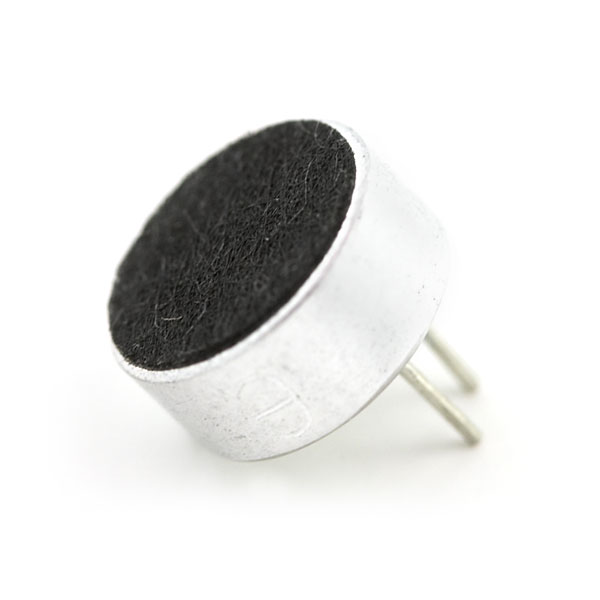
\includegraphics[width=0.4\textwidth]{figures/sscondesermic.jpg}}
\caption{Condeser Microphone}
\label{condesermic}
\end{figure}

Sensor suara merupakan sensor yang mensensing besaran suara untuk diubah menjadi besaran listrik. Sensor ini bekerja berdasarkan besar kecilnya kekuatan gelombang suara yang diterima. Dimana gelombang suara tersebut mengenai membran sensor, yang menyebabkan bergeraknya membran sensor yang memiliki kumparan kecil sehingga menghasilkan besaran listrik. Kecepatan bergeraknya kumparan kecil tersebut menentukan kuat lemahnya gelombang listrik yang akan dihasilkan. Salah satu contoh komponen yang termasuk dalam sensor ini adalah condeser microphone atau mic. Bentuk fisik dari condeser mic yaitu berbentuk bulat dan memiliki kaki dua seperti contoh pada gambar \ref{condesermic}.

\section{Prinsip Kerja Condeser Microphone}

\begin{figure}[ht]
\centerline{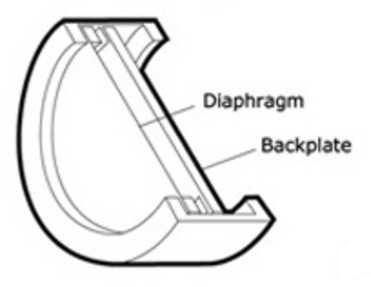
\includegraphics[width=0.4\textwidth]{figures/sscondesermicscheme.jpg}}
\caption{Skema dari Condeser Microphone}
\label{condesermicscheme}
\end{figure}

Condenser mic bekerja berdasarkan diafragma atau susunan backplate yang harus tercatu oleh listrik membentuk sound-sensitive capacitor. Gelombang suara yang masuk ke microphone akan menggetarkan komponen diafragma ini. Letak dari diafragma ditempatkan di depan sebuah backplate. Susunan dari elemen ini membentuk sebuah kapasitor yang biasa disebut juga kondenser. Kapasitor memiliki kemampuan untuk menyimpan muatan maupun tegangan. Ketika elemen tersebut terisi dengan muatan, medan listrik akan terbentuk di antara diafragma dan backplate, yang dimana besarnya itu proporsional terhadap ruang yang terbentuk diantaranya. Variasi akan lebar space antara diafragma dengan backplate terjadi dikarenakan adanya pergerakan diafragma relatif terhadap backplate yang disebabkan oleh adanya tekanan suara yang mengenai diafragma. Hal ini akan menghasilkan sinyal elektrik dari gelombang suara yang masuk ke condenser microphone seperti contoh pada gambar \ref{condesermicscheme}.

\section{Karakteristik dari Condeser Microphone}

\hspace{4mm} Karakteristik dari Conseder Microphone adalah sebagai berikut :

\begin{itemize}
\item Susunannya lebih kompleks dibanding dengan jenis microphone lainnya seperti dibanding dengan dynamic Microphone.
\item Pada frekuensi tinggi, akan menghasilkan suara yang lebih halus dan natural, serta sensitivitas yang lebih tinggi.
\item Mudah akan mencapai respon frekuensi flat dan memiliki range frekuensi yang lebih luas.
\item Ukurannya lebih kecil dibanding dengan jenis tipe mikrophone lainnya.
\end{itemize}

Pada pasaran sudah dijual sensor suara menggunakan condeser mic ini dalam bentuk modul, sehingga mudah dan praktis dalam penggunaannya.

\section{Spesifikasi dari Modul Sensor Suara}

\begin{figure}[ht]
\centerline{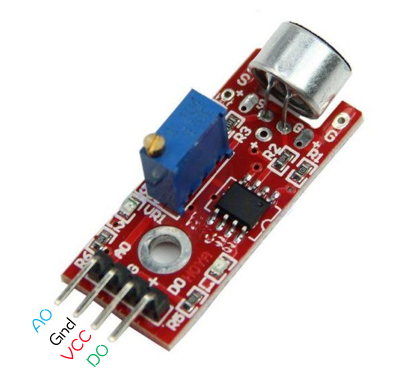
\includegraphics[width=0.4\textwidth]{figures/sssensorsuara.png}}
\caption{Modul Sensor Suara}
\label{sssensorsuara}
\end{figure}

Spesifikasi dari modul sensor suara seperti contoh pada gambar \ref{sssensorsuara} adalah sebagai berikut :

\begin{itemize}
\item Sensitivitas dapat diatur (pengaturan manual pada potensiometer).
\item Condeser yang digunakan memiliki sensitivitas yang tinggi.
\item Tegangan kerja antara 3.3V – 5V.
\item Terdapat 2 pin keluaran yaitu tegangan analog dan digital output.
\item Sudah terdapat lubang baut untuk instalasi.
\item Sudah terdapat indikator led.
\end{itemize}

\section{Tutorial Mengakses Sensor Suara}

\hspace{4mm} Bahan-bahan yang diperlukan untuk mengakses sensor suara, yaitu :

\begin{itemize}
\item Arduino Uno R3
\item Komputer + Software IDE Arduino
\item Modul Sensor Suara
\item Kabel Jumper
\item Lampu LED
\item Kabel USB
\end{itemize}

\break Proses pembuatan :

\begin{enumerate}

\item  Pertama, pasang kabel jumper bagian female ke masing-masing pin modul sensor suara. Kabel jumper berwarna putih ke pin Analog Output (AO). Kabel jumper berwarna abu-abu ke pin Ground (G). Kabel jumper berwarna hitam ke pin Voltage Common Collector (VCC)/+.
\break
\centerline{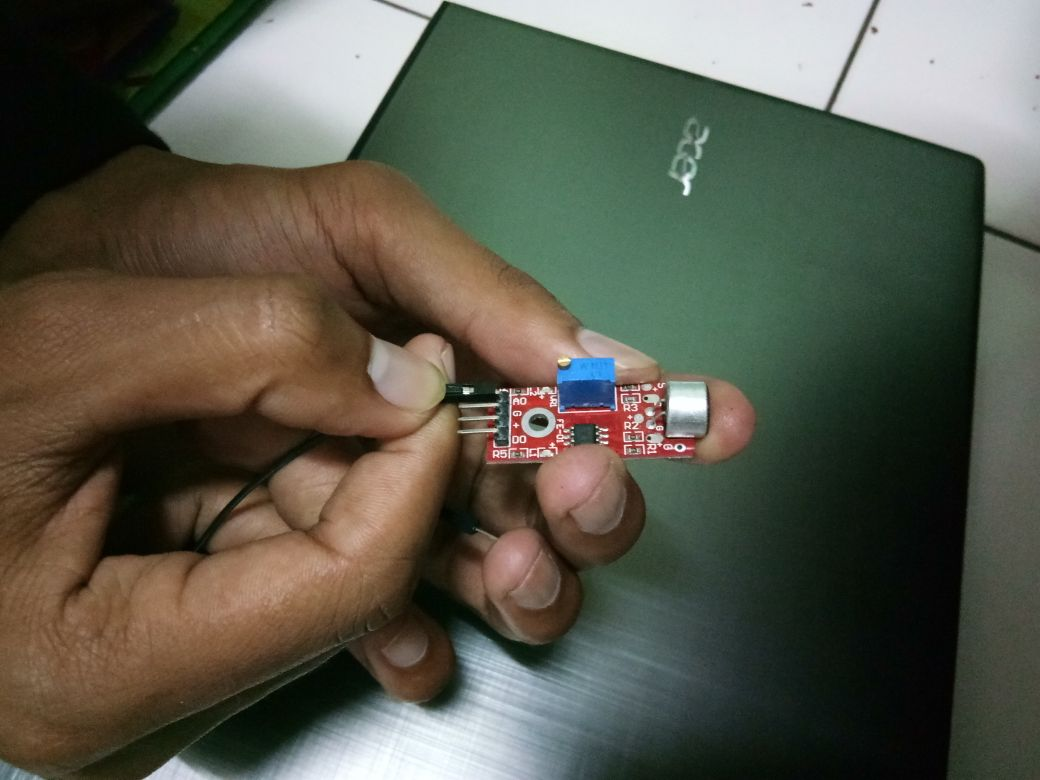
\includegraphics[width=0.9\textwidth]{figures/ss4.jpeg}}
\break
\centerline{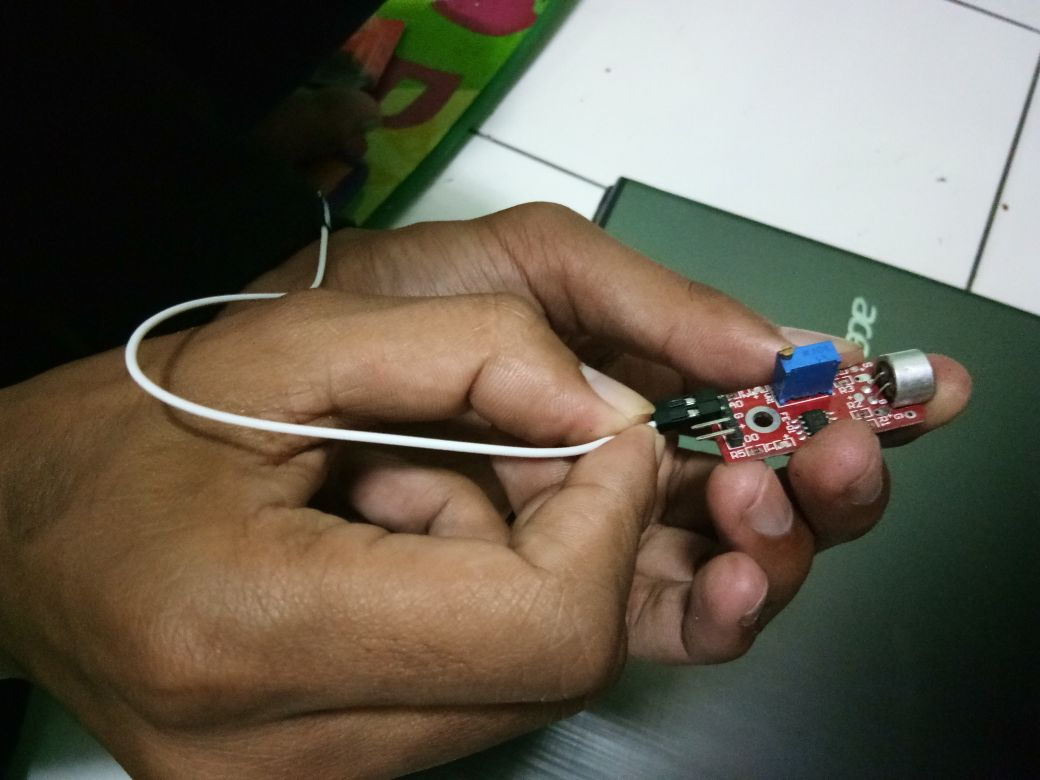
\includegraphics[width=0.9\textwidth]{figures/ss5.jpeg}}
\break
\centerline{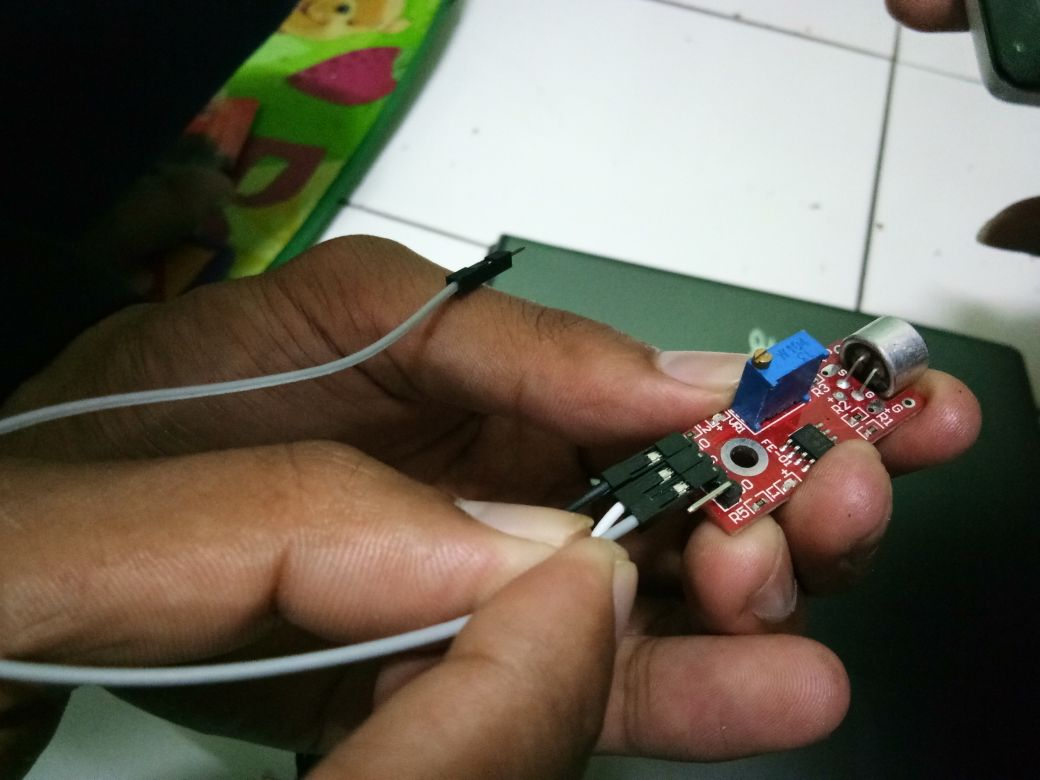
\includegraphics[width=0.9\textwidth]{figures/ss6.jpeg}}
\item Setelah semuanya terpasang, lalu sambungkan kabel jumper bagian male ke arduino. Kabel jumper berwarna putih ke slot A2. Kabel jumper berwarna abu-abu ke slot GND. Kabel jumper berwarna hitam ke slot 5V.
\break
\centerline{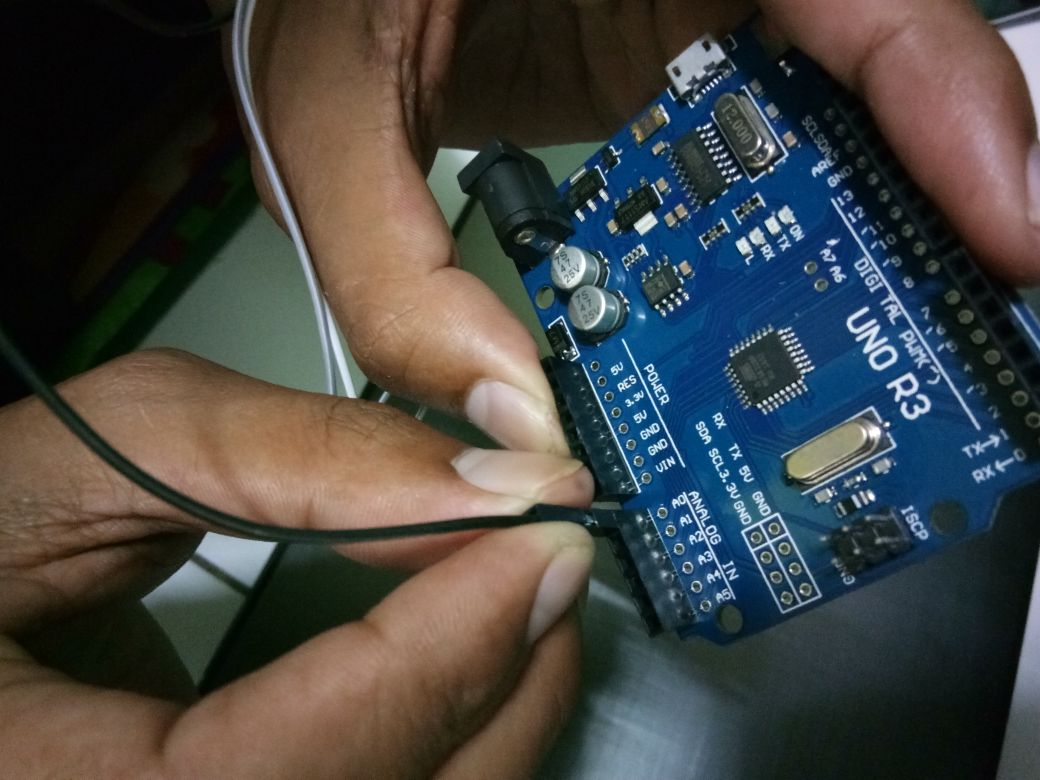
\includegraphics[width=0.9\textwidth]{figures/ss1.jpeg}}
\break
\centerline{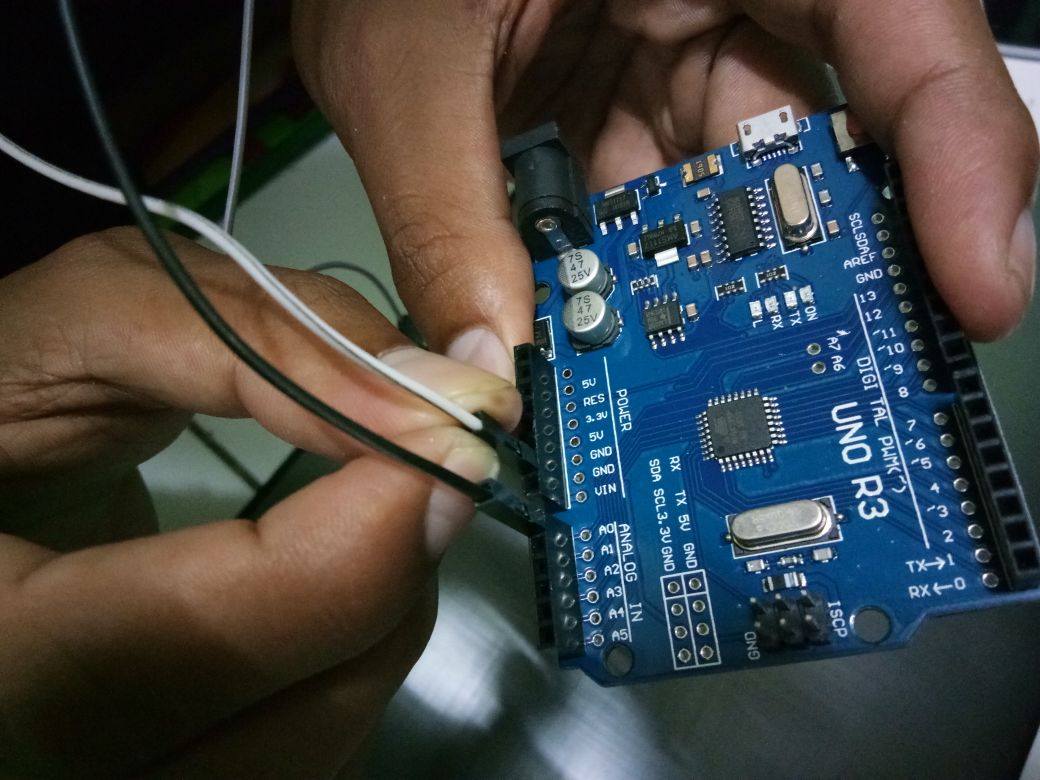
\includegraphics[width=0.9\textwidth]{figures/ss2.jpeg}}
\break
\centerline{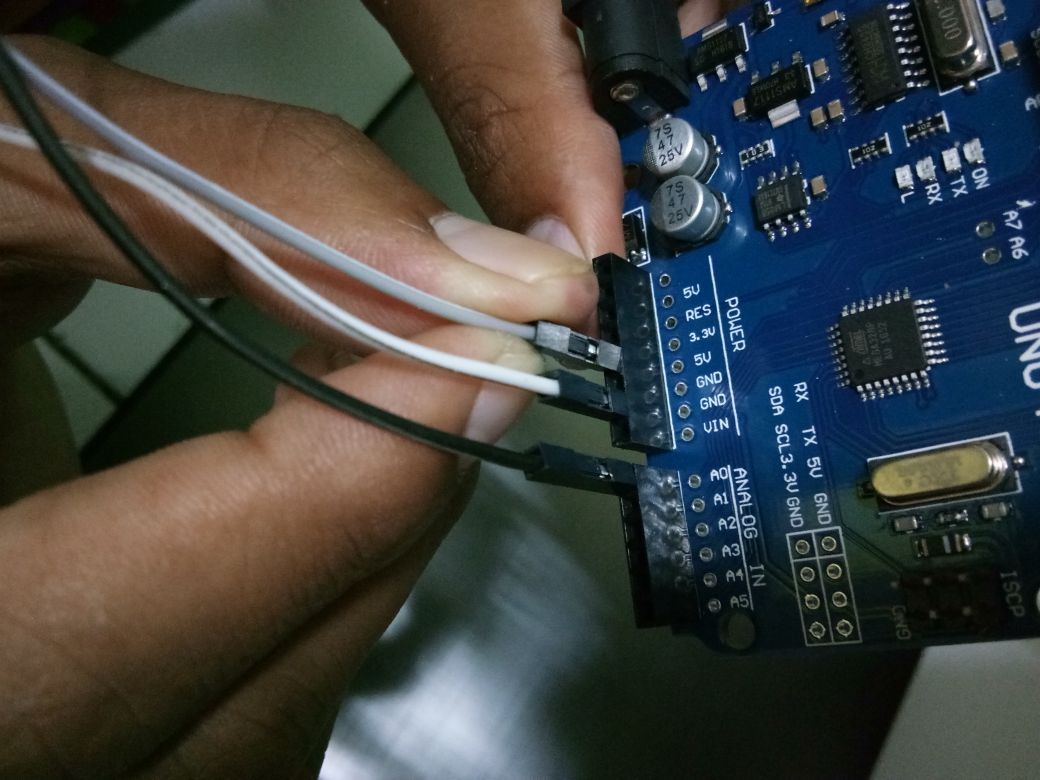
\includegraphics[width=0.9\textwidth]{figures/ss3.jpeg}}
\item Setelah semua terhubung, lalu sambungkan kabel USB ke arduino dan ke komputer.
\break
\centerline{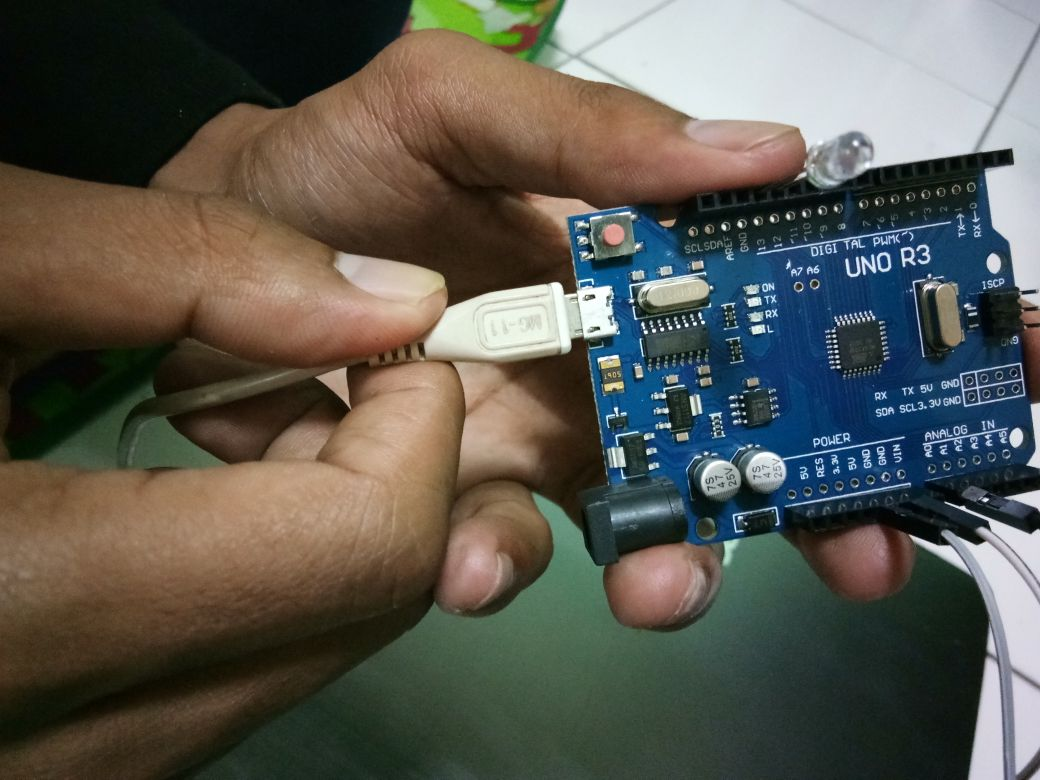
\includegraphics[width=0.9\textwidth]{figures/ss8.jpeg}}
\break
\centerline{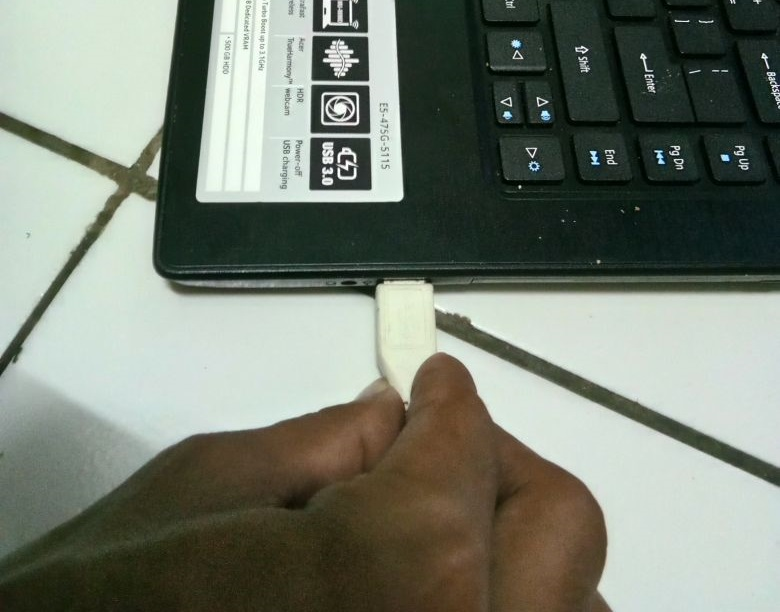
\includegraphics[width=0.9\textwidth]{figures/ss7.jpeg}}
\item Lalu pasang lampu LED ke arduino. Pin yang lebih panjang pasang ke slot 13, sedangkan pin yang pendek pasang ke slot GND.
\break
\centerline{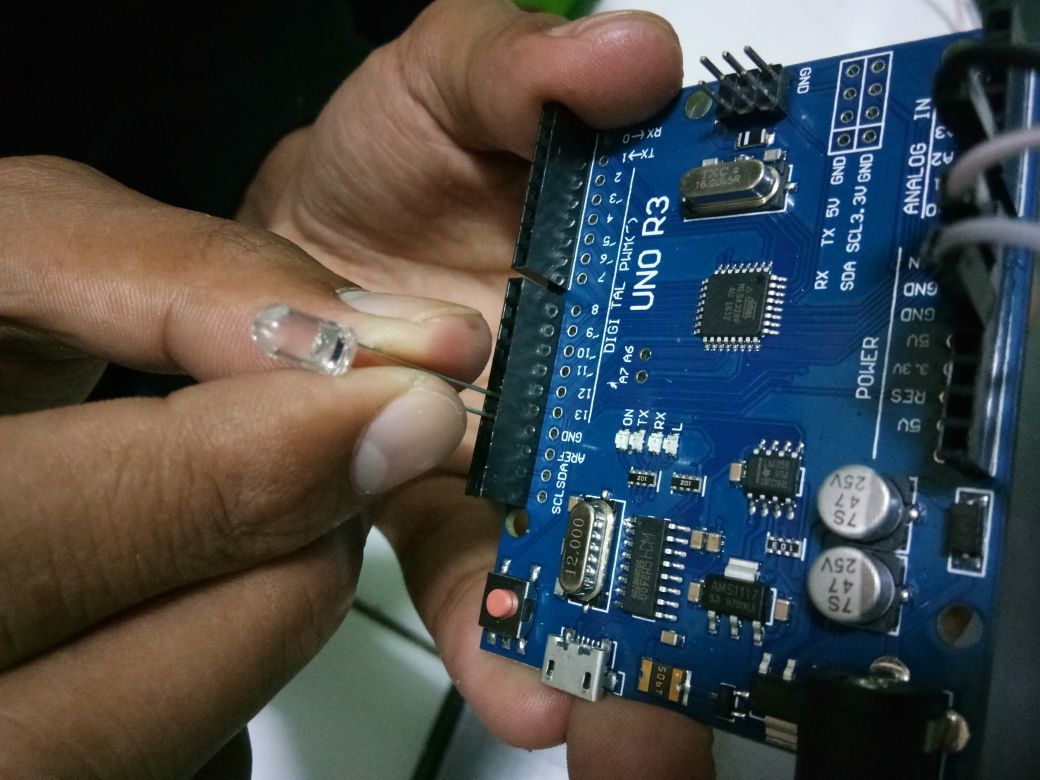
\includegraphics[width=0.9\textwidth]{figures/ss9.jpeg}}
\item  Kemudian buat program yang nantinya digunakan untuk mengetes sensor menggunakan IDE Arduino.
\break
\centerline{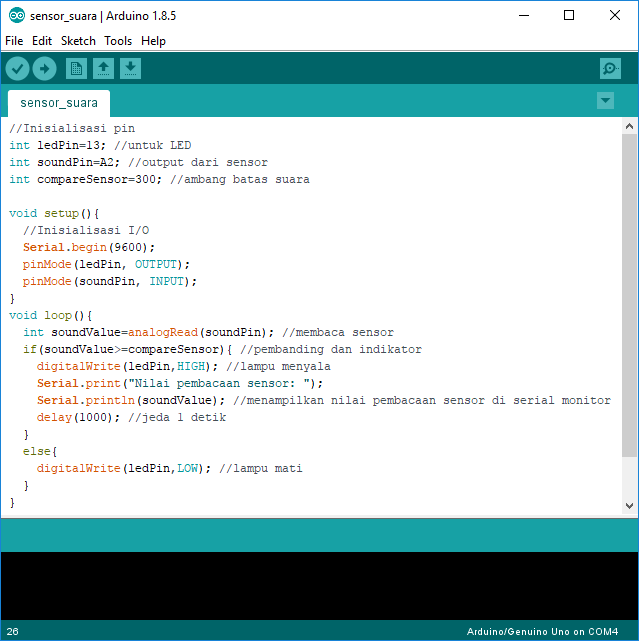
\includegraphics[width=0.9\textwidth]{figures/ss10.png}}
\item Lalu setelah program selesai dibuat, unggah program tersebut ke arduino.
\break
\centerline{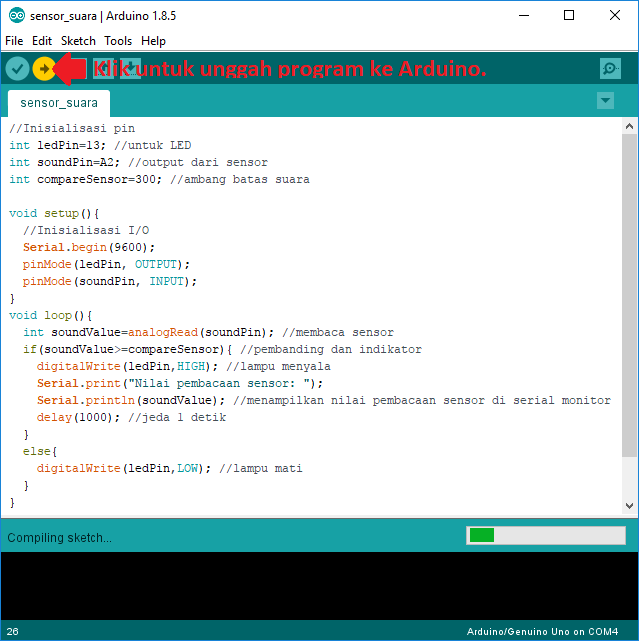
\includegraphics[width=0.9\textwidth]{figures/ss11.png}}
\item Terakhir cek apakah sensor berkerja dengan semestinya.
\break
\centerline{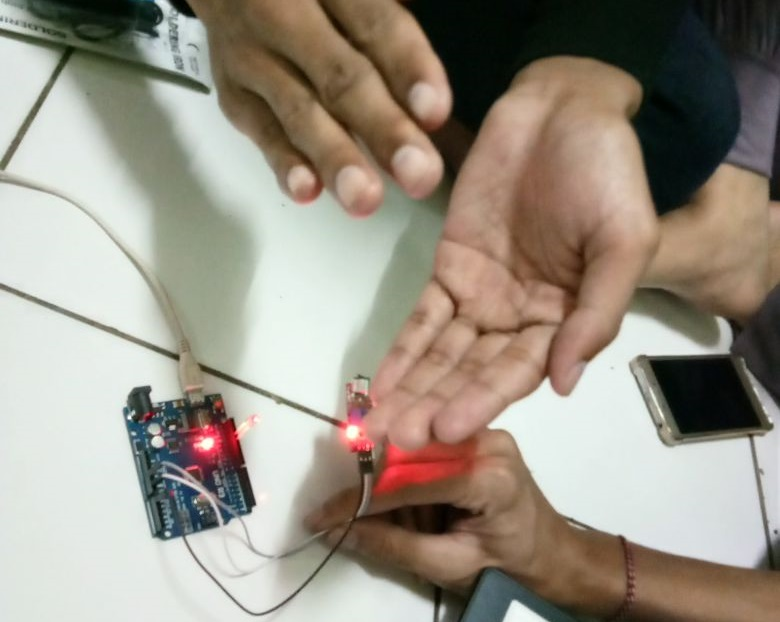
\includegraphics[width=0.9\textwidth]{figures/ss12.jpeg}}
\break
\centerline{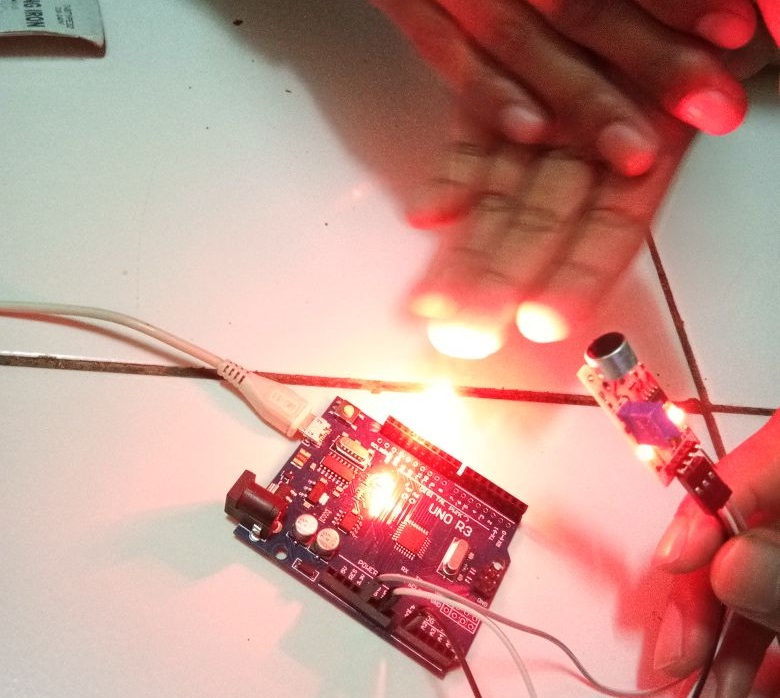
\includegraphics[width=0.9\textwidth]{figures/ss13.jpeg}}
\item Untuk mengecek nilai yang ditangkap oleh sensor, cek pada Serial Monitor.
\break
\centerline{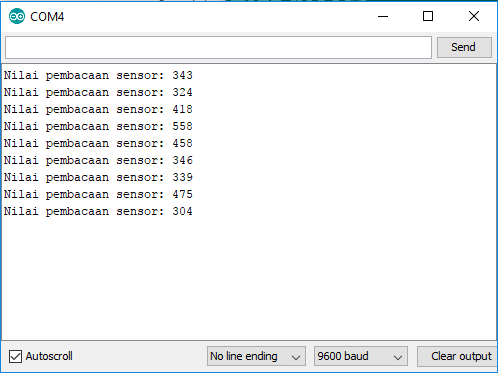
\includegraphics[width=0.9\textwidth]{figures/ss14.png}}

\end{enumerate}

%\end{document}